\documentclass[12pt,a4paper,twoside]{article}
\usepackage{fancyhdr,graphicx,latexsym}

\setlength{\parindent}{0cm}
\setlength{\parskip}{2ex plus1ex minus 0.5ex}

\addtolength{\evensidemargin}{-2.5cm}
\addtolength{\oddsidemargin}{-0.5cm}
\addtolength{\textwidth}{3cm}

\addtolength{\headheight}{0.2cm}
\addtolength{\topmargin}{-1cm}
\addtolength{\textheight}{2.5cm}

\renewcommand{\_}{\texttt{\symbol{95}}}
\addtolength{\fboxsep}{0.1cm}
\newcommand{\param}[1]{\textit{\textrm{\textmd{#1}}}}
\newcommand{\codebar}{\rule{\textwidth}{0.3mm}}
% \newcommand{\spc}{\hspace{0.5mm}$\sqcup$\hspace{0.6mm}}
\newcommand{\spc}{\hspace{0.5mm}$\Box$\hspace{0.5mm}}
\newcommand{\todo}[1]{\textbf{TODO: #1}}

\newlength{\codelen}
\newcommand{\code}[1]
{\begin{center}\fbox{\parbox{16cm}{\texttt{#1}}}\end{center}}

\fancyhead{}
\fancyhead[RO,LE]{\thepage}
\fancyhead[LO,RE]{PIRATES Component Middleware Overview}
\fancyfoot{}
\pagestyle{empty}

\newenvironment{bulletlist}
{
	\begin{itemize}
	\setlength{\itemsep}{0ex}
	\setlength{\parsep}{0ex}
}
{
	\end{itemize}
}

\newenvironment{alphalist}
{
	\begin{enumerate}
	\setlength{\itemsep}{0ex}
	\setlength{\parsep}{0ex}
	\renewcommand{\labelenumi}{(\alph{enumi})}
}
{
	\end{enumerate}
}

\newenvironment{numericlist}
{
	\begin{enumerate}
	\setlength{\itemsep}{0ex}
	\setlength{\parsep}{0ex}
}
{
	\end{enumerate}
}

\begin{document}

% \sfseries
\centerline{\textbf{\LARGE PIRATES Component Middleware Overview}}
\begin{center} \large
David Ingram\\
TIME-EACM Project\\
University of Cambridge Computer Lab\\
12th August 2009\\
\end{center}

{ \parskip 0.1mm plus 0.1mm \tableofcontents }
\pagestyle{fancy}
\newpage

\section*{Glossary}
\addcontentsline{toc}{section}{Glossary}

\begin{tabular}{l@{\ --\ }l}
\textbf{PIRATES} & Peer-to-peer Implementation of Reconfigurable
	Architecture for Typed Event Streams\\
\textbf{SBUS} & Stream BUS -- the old development name for PIRATES;\\
	& still referred to in the documentation\\
\textbf{IDL} & Interface Definition Language\\
\textbf{LITMUS} & Language of Interface Types for Messages in Underlying Streams\\
\textbf{RDC} & Resource Discovery Component\\
\end{tabular}

\section*{PIRATES Documentation List}
\addcontentsline{toc}{section}{PIRATES Documentation List}

The PIRATES manual is split into a number of different documents, of which this
is the first. The complete list is given below.

%\subsubsection*{Core}
\begin{bulletlist}
\item \textbf{PIRATES Component Middleware Overview} -- this document
\item \textbf{PIRATES User Guide} -- how to install and operate it
\item \textbf{PIRATES C++ Binding}
\item \textbf{PIRATES Java Binding}
\item \textbf{PIRATES Data Representation} -- the type system
\item \textbf{PIRATES Protocol} -- for internal developers only
\end{bulletlist}
%\subsubsection*{Future add-ons} (out of date)
%\begin{bulletlist}
%\item \textbf{SBUS Prebuilt Components}
%\item \textbf{SBUS Extensions}
%\item \textbf{SBUS Dynamics}
%\item \textbf{SBUS Hackers Guide}
%\item \textbf{SBUS Python Binding} -- TBA
%\end{bulletlist}
%\subsubsection*{Internal use only}
%\begin{bulletlist}
%\item SBUS Requirements
%\item SBUS TODO List
%\item SBUS Implementation Notes
%\end{bulletlist}

\newpage

\section{Introduction}

PIRATES is a component-based \textit{middleware} which makes it easier to
write large-scale
networked programs in C++ or Java. It is particularly suitable for
applications which process streams of data from networks of sensors.
It comprises an underlying communication protocol and type system,
a component wrapper program, libraries for component development in
the target languages, and utility programs to manage the network.

The key features provided by PIRATES are \textit{integrated messaging,
peer-to-peer communication, decoupling, events, dynamic reconfiguration,
type checking, resource discovery and a simple API.}

\textbf{Integrated Messaging:} PIRATES lets you perform RPCs and
message passing within the same framework, so you don't need
two different libraries to access services and to send continuous
media streams.\\
\textbf{Peer-to-Peer Communication:} Messages are sent directly
between peers, with no fixed servers or brokers required.
This makes it a decentralised architecture, with no central
bottlenecks as the system grows.\\
\textbf{Decoupling:} With a centralised system, sources and
sinks can be decoupled, so that neither need be aware of the identity
of the others.
PIRATES uses wrapper processes which monitor the P2P links,
providing the same decoupling benefits whilst actually transferring
data point to point. For example, if one component disconnects, the wrapper
can reconnect to an alternative without the application
having to deal with the error.\\
\textbf{Events:} Components may set up subscriptions which filter
the events they receive. An optional event broker provides
message aggregation for publish-subscribe operation.\\
\textbf{Dynamic Reconfiguration:}
The links between components can be reconnected at any time in a live
system by any other component. Hence managers and load balancers
can reconfigure to cope with change, without stopping or restarting the
running components.
The connection information resides in configuration files, so it
can be changed much more flexibly than clients which are internally
programmed to connect to a specific server.\\
\textbf{Type Checking:}
All messages are structured and typed, being essentially XML documents.
For efficiency there is however a binary transport layer.
The range of valid types are described by message schemas.
Type checking ensures that clients are always mapped to servers
with compatible message types.\\
\textbf{Resource Discovery:}
Components are self-documenting and reflective.
Resource discovery components (RDCs) are used to help locate them.
All components can be queried for their identity, schemas, status
and the locations of peer components, so the web of components
can be explored.\\
\textbf{Simple API:}
PIRATES has a simple, lightweight API which combines well with
other libraries. It does not create
any threads within the application's process, impose its own build
system, nor does it take over the thread of control with its own event loop.
It integrates cleanly with other I/O using the standard \verb^select()^
or \verb^Selector^ mechanisms. It has no external dependencies.\\

\section{Communication sequences}

PIRATES has two general modes for communication between each linked
pair of components. Interactions with replies (such as RPC) are
dealt with by \textbf{client} and \textbf{server} endpoints.
Those without replies
are handled by \textbf{source} and \textbf{sink} endpoints.

Clients and servers must be connected to each other, and likewise
for sources and sinks. The client-server mapping is many-one and
the source-sink mapping is many-many (so a source may send
data to multiple sinks, each of which is receiving data from multiple
sources).

%\begin{figure}[h]
%\centering
%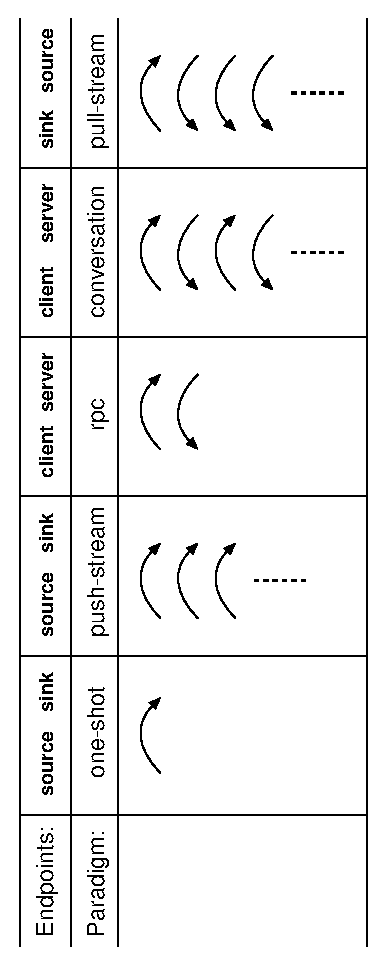
\includegraphics[scale=1.0,angle=-90]{diagrams/arrows.eps}
%\caption{Use case diagrams for the four endpoint types}
%\label{usecases}
%\end{figure}

%Figure \ref{usecases} shows how the four endpoint types enable a complete
%range of familiar communication paradigms.
%RPCs follow the familiar request-reply pattern.
%The ``conversation'' entry in the diagram covers
%protocols such as negotiation or handshakes where connection
%state is stored at both ends (unlike a sequence of disjoint RPCs),
%such as in online shopping transactions.
%Less regular interactions, involving several messages sent one way before
%the other can be cast into the form of a conversation by inserting null
%acknowledgement messages.
%The column labelled pull-stream is
%suitable for \textit{publish-subscribe} architectures (actually
%this part of it is \textit{subscribe-notify}, and event \textit{publishing}
%is covered by the push-stream case).

\begin{center}
\begin{tabular}{|l|c|c|}
\hline
\textbf{Communication mode} \rule[-2mm]{0mm}{6.5mm} &
\textbf{Streams} & \textbf{RPC}\\
\hline
Active endpoint \rule[0mm]{0mm}{4.5mm} & source & client\\
Passive endpoint & sink & server\\
Message type & event & query\\
Response type: \rule[-2mm]{0mm}{2mm} & N/A & reply\\
\hline
\end{tabular}
\end{center}
\vspace{2mm}

Note that any component can be both a user of multiple
streams and RPC services as well as providing services to other components.
There can also be multiple connections with different modes between
the same pair of components.

\section{Type system}

All messages sent by PIRATES must adhere to a schema. The schema for
a particular kind of message is written in the LITMUS schema language.
Each schema is also passed through a hash function, which generates
a 6 byte value called the LITMUS code.
Before hashing, the schema is normalised (all white
space and comments are removed).
The code is then used to label all
messages conforming to that schema when sent across the network,
or if stored on disk. When a component receives a message, it
can compare the LITMUS code with the one it expects for that connection.

This is safer than using a type ID or version number because it gives
some assurance that the correct API is being programmed to.
An application programmer will embed the hash value of the
API they are assuming in their code; this is then checked for
them by the library and an error raised if the packets
received do not match.

Polymorphic components (such as the event broker) accept messages
of different types. In this case, any LITMUS code may be
accepted. The code is checked against the schemas which the
receiving component has seen before and stored in its schema cache.
If it isn't recognised, the sender is queried to provide the full
schema. This ensures that all components have the schemas of
the messages they receive available, but for most messages the
overhead is just 6 bytes for the LITMUS code.

\section{Architecture}

\begin{center}
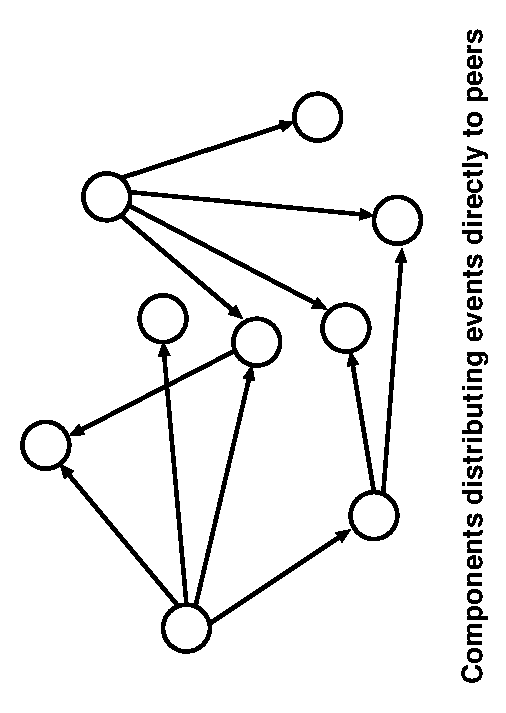
\includegraphics[scale=0.7,angle=-90]{diagrams/decentralised.eps}
\end{center}

PIRATES is a peer-to-peer architecture in which every component possesses
event multicasting abilities. Each component can register
subscribers for the events it generates, and distributes event
notifications in a one-to-many fashion to them. There are no
intermediaries unless you explicitly choose to use the separate broker
component; messages are normally sent from source
to destination in a single step. Provisioning for large numbers of
clients can be handled by several levels of fan out.

Removing the requirement for a central event broker benefits
scalability and removes a central point of failure. A resource
discovery component is still needed to locate components, although
there may be more than one of these and they are not on the data path.

One disadvantage of this architecture is an increase in the complexity
of each individual component. A further drawback is that subscribers
are not fully decoupled from data sources, hence clients must deal with
required components not existing when they start up, and perform
reconnection if an event source is stopped and restarted. PIRATES avoids
both of these problems with its use of component wrappers,
described below.

PIRATES requires TCP/IP. Normally a process will implement one
component. Any number of components can run on a single machine.

\section{Component wrappers}

% \begin{figure}[htbp]
\begin{figure}[h]
\centering
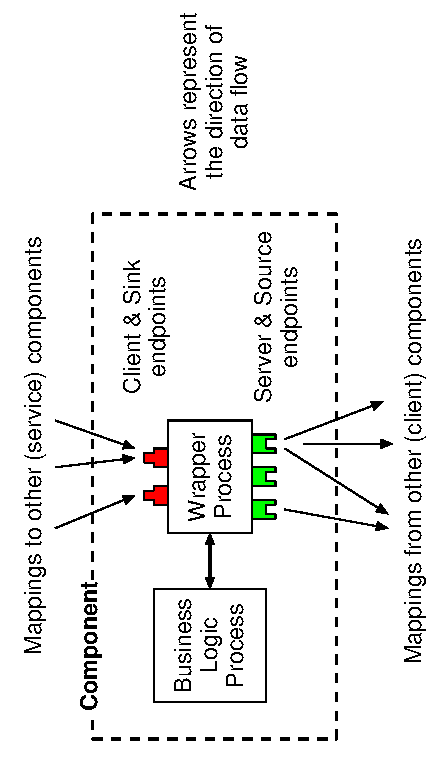
\includegraphics[scale=1.0,angle=-90]{diagrams/parts.eps}
% \caption{Foo}
% \label{proxies}
\end{figure}

Wrappers are implemented as separate processes.
The same wrapper program is used for all components, whether pure
servers, pure clients, or
hybrid server/clients. The latter is common since a stream
sink is often also a stream source, and a service is often a
client of another component.
Pure clients are treated as components which may not be registered with
a RDC and happen to have no server or source endpoints.

The wrapper program is written in C++, forked from the application's
business logic process by the PIRATES library, and communicates with it
via a number of pipes (one bidirectional pipe for each endpoint, plus
a bootstrap connection). The wrapper can make progress on any number of
connections concurrently, and for robustness it achieves this with a
single-threaded fully non-blocking design.

The business logic process is free to use a single or multi-threaded
design as the component author sees fit.

For data producers, the functions of the wrapper include handling
subscriptions and sending notifications.
For consumers, the wrapper ensures that
stream sink implementations do not have to deal with retry and
reconnection themselves when a service dies or is initially unavailable.
The wrapper handles streams subscribed to and emits silence instead of
an error when streams are unavailable.

\section{Endpoints}

Each component can offer multiple services, each of which is
selected by a named endpoint of type server or source.
Each endpoint has a different
schema for queries and replies. The component metadata
includes these, so the definitions are available for you to inspect.

Connections to a component are made to its network address
(IP and port number). The endpoint is then specified over the
connection to identify precisely which service is required.

Endpoints are also the abstraction which applications use to describe
the services they need. By avoiding hardcoded connections to
specific components we can better support
dynamic reconfiguration and features such as component migration.

An endpoint is defined to support a given set of API hashes.
Having defined the endpoint, an application may perform I/O with it
immediately. At any time, third parties can
\textit{remap} the endpoint using the built-in endpoint provided by
the application's wrapper for that purpose, in order to connect
it with another component. Optionally, the component itself
may \textit{map} the endpoint, if it knows what to connect it to.
Pairs of endpoints to be mapped together do not have to have the same name,
but their schemas must match and their endpoint types must be complementary.

\section{Naming}

Components names are unstructured ASCII strings. They do not have to
be unique. Simple component names such as
\verb^traffic^, \verb^clean^, \verb^filter^, \verb^carparks^,
\verb^anon^, \verb^select^, \verb^weather^, \verb^archive^ or
\verb^summary^ are preferred over complex ones such as\\
\verb^filtered-pseudonymised-aggregate-gps^, since the latter
information is better expressed by the connections between simple
components.
The purpose of names is mainly to assist humans in
visualising the system.

Components to address are described to RDCs by a list of
criteria, not just the name. This allows for example picking from
a number of identically-named standard filter components the one
connected to a specific data source.

Any subset of the following component selection criteria
may be used:
\begin{bulletlist}
\item Component name.
\item Message schema hashes.
This criterion is \textit{always} used, to ensure only
compatible pairs of endpoints are connected.
\item Direct or indirect peer components.
\item Public key (guarantees identity).
\item Component author.
\item Other keywords.
\item An explicit host and port location.
\end{bulletlist}

RDCs maintain this information for all components which have registered
with them. Components are not required to keep a TCP connection to
the RDC open for this purpose; instead the RDC pings them peridiocally.
The RDC also publishes a stream of updates to liveness information.

\end{document}
